% !TeX TS-program = pdflatex
\documentclass[xcolor={svgnames,x11names}]{beamer}

\makeatletter
\setlength\beamer@paperheight{12.096cm}%
\geometry{papersize={\beamer@paperwidth,\beamer@paperheight}}
\beamer@calculateheadfoot
\makeatother

\usepackage{tikzlings}
\usepackage{tikzducks}
\usepackage{pdfpages}
\usetikzlibrary{positioning,shapes}
\usetikzlibrary{overlay-beamer-styles}

\usepackage[osf]{AlegreyaSans}
\usepackage{array}
\graphicspath{{images/}}

\setbeamertemplate{navigation symbols}{}
\setbeamercolor{background canvas}{bg=Seashell1}


\begin{document}

\begin{frame}
\LARGE\sffamily
\bfseries\scshape
\centering  A Tikzducks Production

\fontsize{14.4}{16pt}\selectfont
\bigskip

\begin{tabular}{*{2}{>{\centering}p{0.44\linewidth}}}
\multicolumn{2}{c}{Graphics, Animations, Video and Sound}\tabularnewline[5pt]
SamCarter &  Ulrike Fischer \tabularnewline
\vspace{0pt}
\includegraphics[width=0.65\linewidth,keepaspectratio]{samcarter-avatar}
&\vspace{0pt}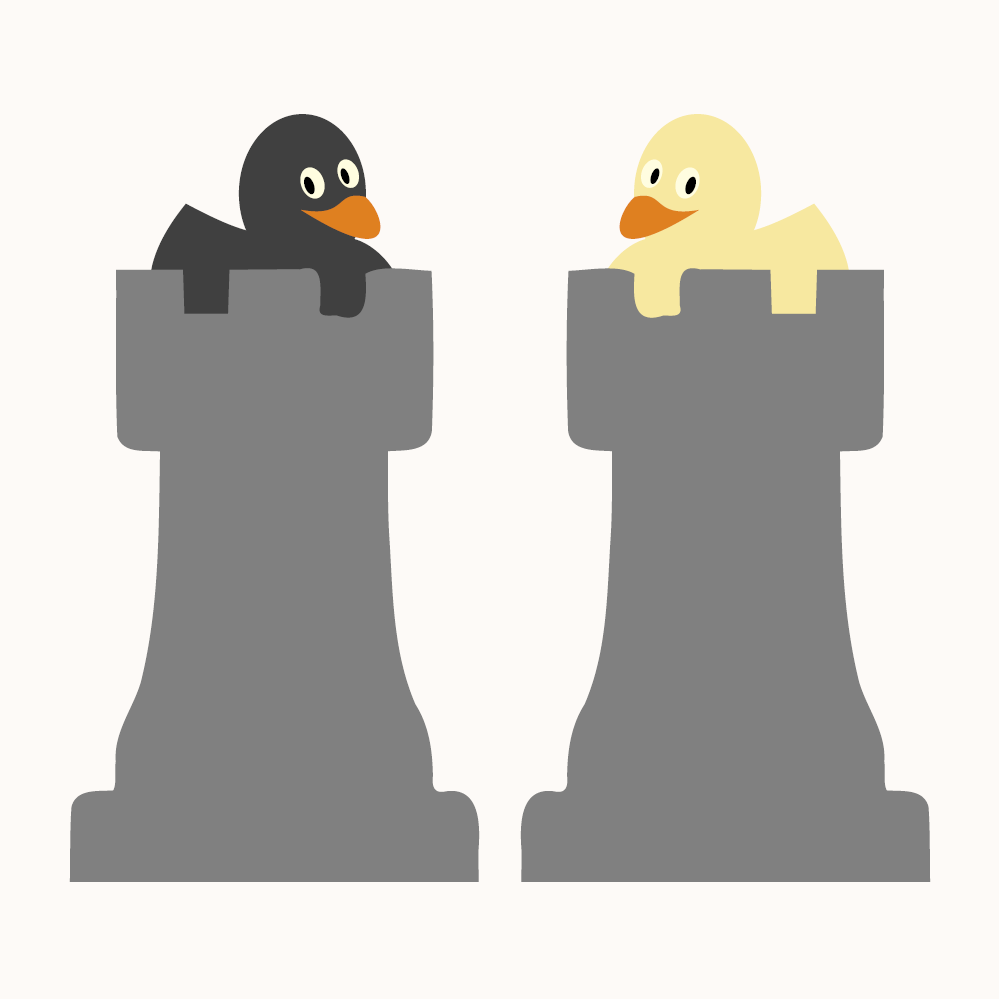
\includegraphics[width=0.65\linewidth,keepaspectratio]{ulrike-avatar}
\end{tabular}

\medskip
\begin{tabular}{*{2}{>{\centering}p{0.44\linewidth}}}
Idea  &Music \tabularnewline
\makebox[0pt][c]{Gert Fischer}      & Richard Wagner
\tabularnewline
\vspace{0pt}
\includegraphics[width=0.65\linewidth,]{gert-avatar}
&\vspace{0pt}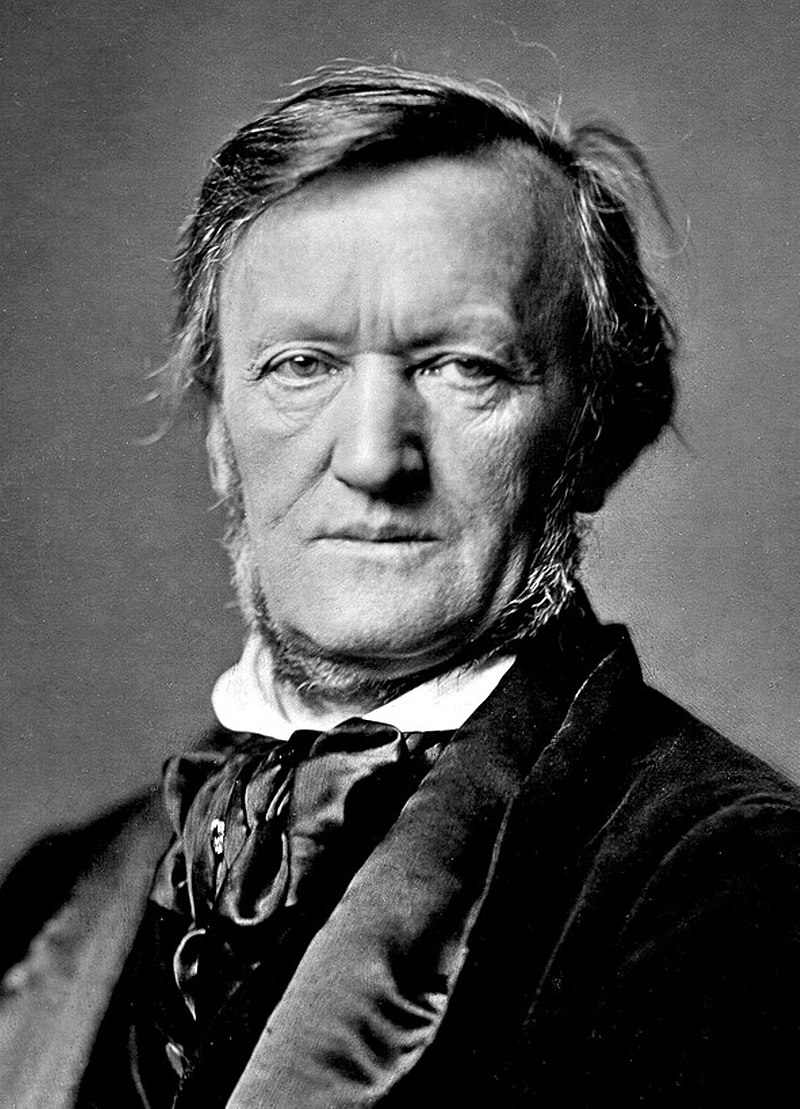
\includegraphics[height=0.6\linewidth]{RichardWagner}

\end{tabular}
\pause[120]
\end{frame}
\end{document}
